
Different prototypes were used to decide, how the program should interact with the user and how the final user interface should be designed. In the following sections three different prototypes will be shown along with our work process and an explanation of our decision making.
The first prototypes were drawings on a blackboard or a piece of paper that were later converted to an HTML prototype. In this process three group members designed the first prototype and presented it to the group. The group discussed points of improvements which led to a new design of the prototype. The HTML prototype was furthermore shown to the kindergarten teacher Kristine Niss-Henriksen in the second interview which is summarized in appendix \vref{sec_interview_birken}.

\section{The first prototypes}
After the first prototype was presented each page was drawn on to the blackboard where the changes were more manageable. One of the first blackboard designs was of the page ``Settings`` which contained information such as the child's name and abilities, shown in Figure \vref{fig:firstProto}. This is a primitive design with two menus one horizontal and one vertical, where the horizontal has all children and groups of children and the vertical has all the applications on a child's device, that the user can administer. This menu will be further explained for the next prototype. 

\begin{figure}[!ht]
	\centering
		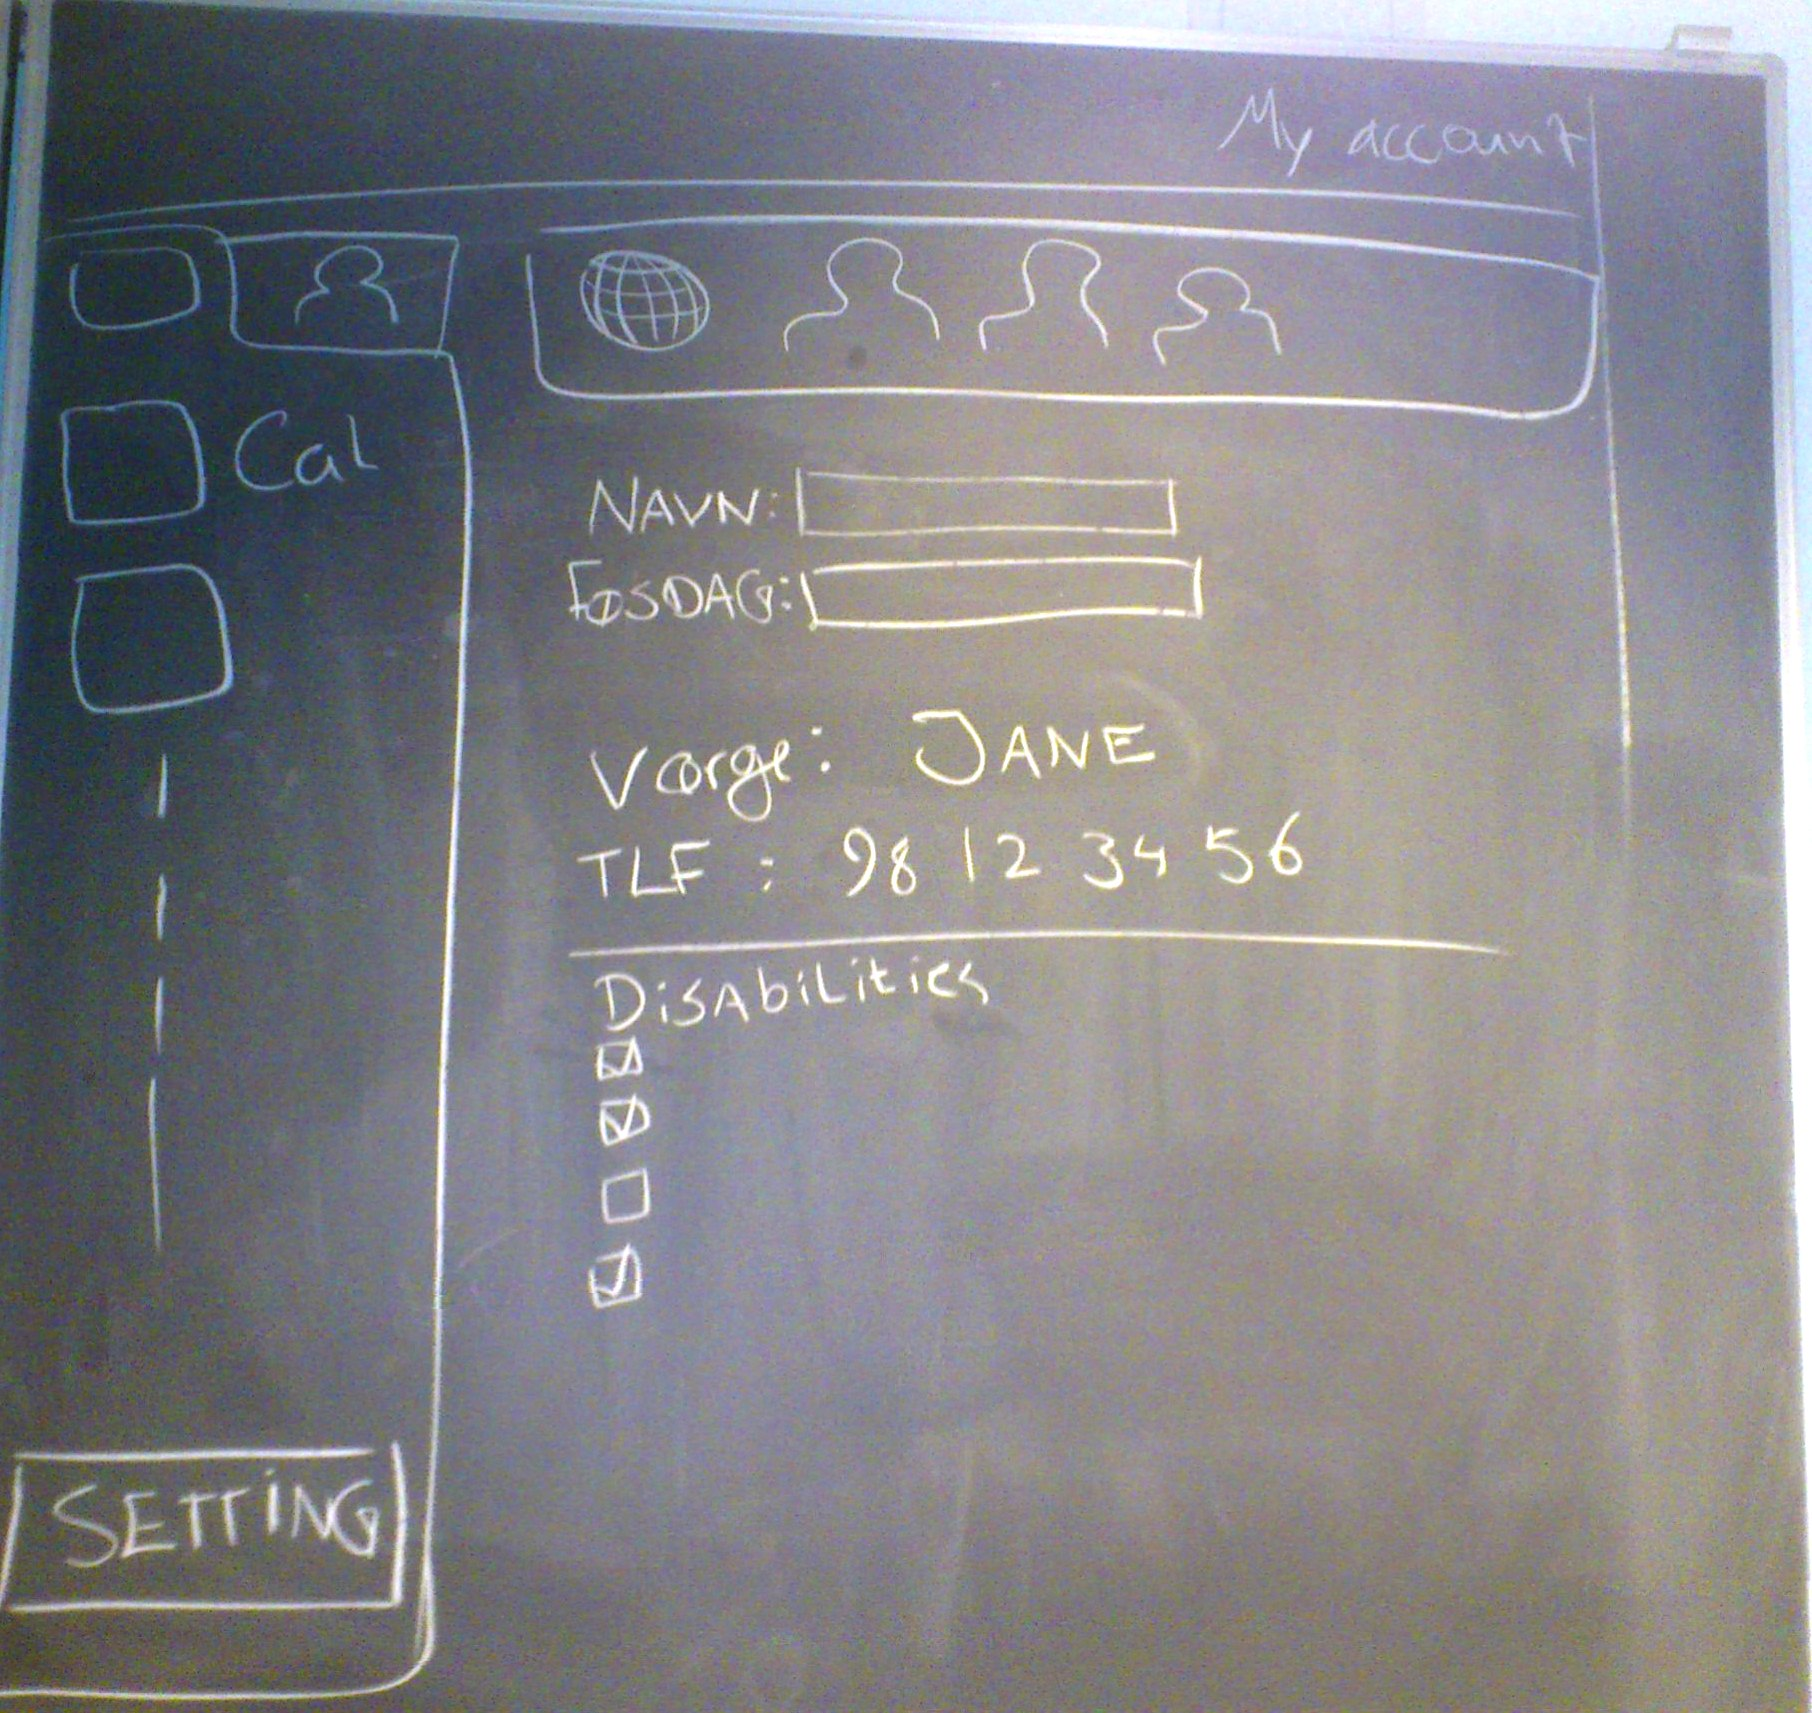
\includegraphics[width=0.60\textwidth]{img/firstproto.jpg}
	\caption{Black board design of the interface}
	\label{fig:firstProto}
\end{figure}


The group members did disagree on how to get into this page, because in this design the user would have to choose a child in the top horizontal menu and the press the Settings button in the vertical menu, which is located among Giraf applications. Especially the location and the naming of the ``Settings`` button were discussed because the user would get the impression that they administer their child like the applications and not be able to change information about the child. To solve this it was suggested that this page should be in ``My Account`` instead; where the user would also be able to change their own personal information. In our prototypes this was not changed until implementation began. %?om det med implementationen passer ved jeg ikke? sp�rg johannes eller se n�r den er f�rdig

\section{The HTML prototype}
For the second interview with Kristine Niss-Henriksen an HTML prototype was made from the primitive prototypes. The Figure \vref{fig:contactbook} is two screen shoots from the child Jack's contact book where the right side of the figure is an light box with an entry from the contact book. The contact book is inspired by a calendar, because for a date it can have some entries that the user can click on and then within a Light box the message and pictures is shown. If the user has not seen the message before, the signal "Ny!" in the right side should be visible. The user is able to fold and unfold the entries for each date, to see or hide the entries in the contact book. 

\begin{figure}[!ht]
	\centering
		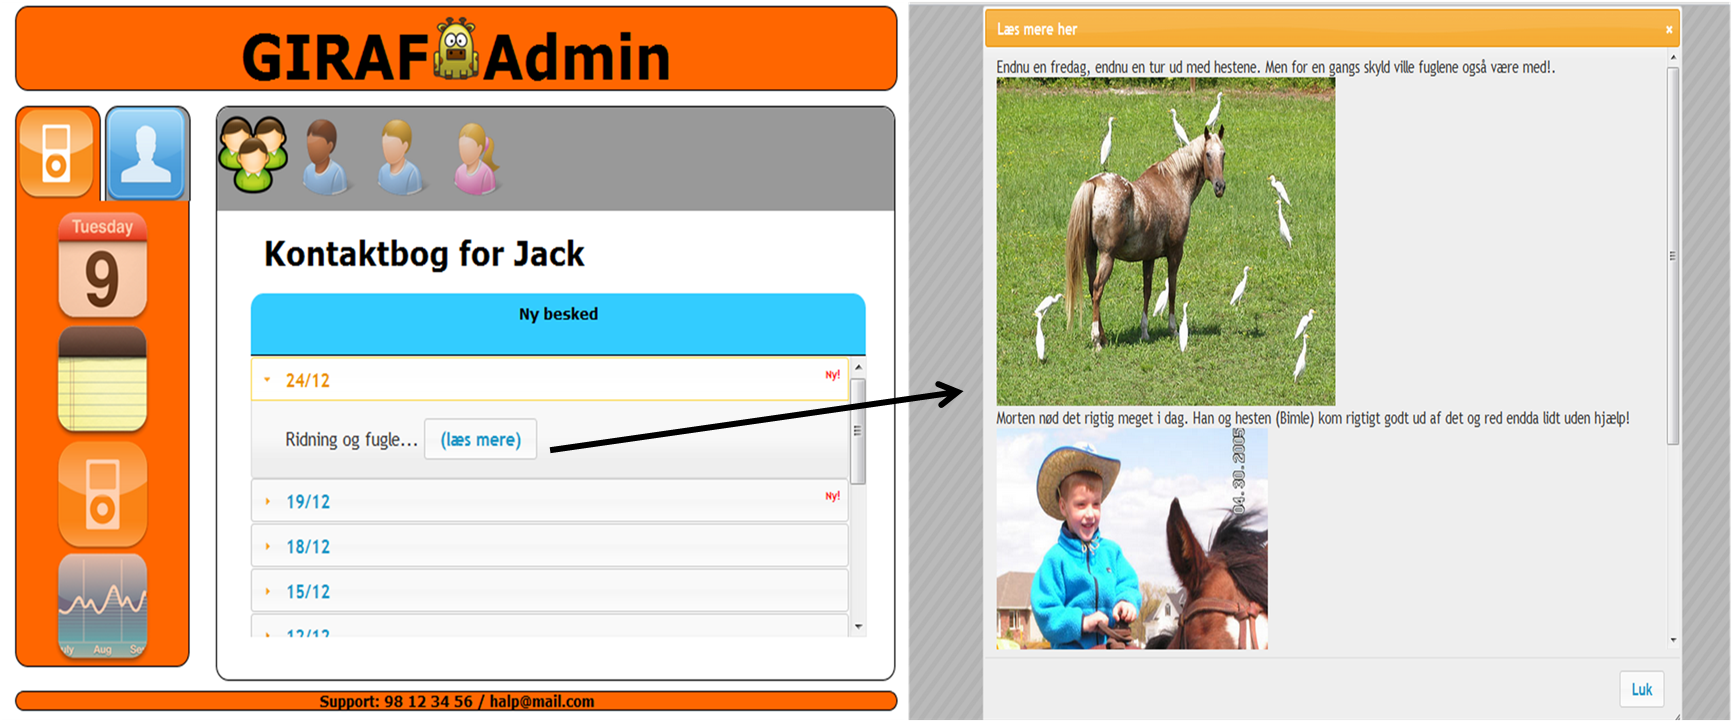
\includegraphics[width=1.00\textwidth]{img/contactbook.png}
	\caption{Prototype of the contact book and the light box with an entry}
	\label{fig:contactbook}
\end{figure}

\subsection{The menus}
As it was pointed out earlier the Giraf applications' administrators is represented on the vertical menu, as an icon that should identify the application administrator. The children's devices are represented on the horizontal menu where the single child's device is identified from a picture and the group is identified by an icon representing a group of children. However this representation can be mirrored such that the children's devices are represented on the vertical menu and the applications are represented on the horizontal menu, which is shown in Figure \vref{fig:menus}. The black circle indicates which of the menus is represented in the vertical menu. This menu was not implemented because it would take too much of the space on the screen, and it could also be a confusing navigation path for the user, without gaining any new functionality. In the next paper prototype this menu was replaced with two vertical menus side by side.

\begin{figure}[!ht]
	\centering
		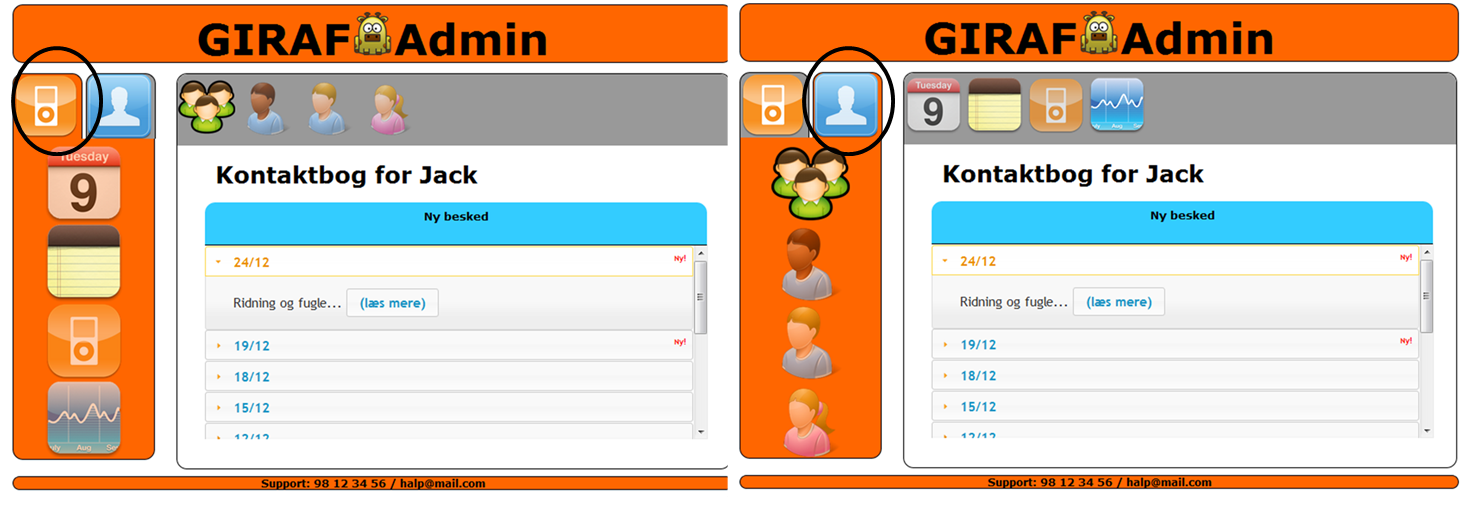
\includegraphics[width=1.00\textwidth]{img/menus.png}
	\caption{The menus in the HTML prototype}
	\label{fig:menus}
\end{figure}


\subsection{Evaluation of the HTML prototype}
In the second interview in appendix \vref{sec_interview_birken} with Kristine Niss-Henriksen from Birken we introduced the HTML prototype to her. In general she liked the design and she commented that the icon for a child should be a photo of the child instead, which also was indented. She also missed a way to make a reply to a message which would be useful since it is used both by the parents and kindergarten teachers. Kristine said: "[communication] \textit{It goes in both directions. The parents write in the contact book in the morning and we write during the afternoon which then can result in a longer dialog between the parties.}" in appendix \vref{sec_interview_birken} [12:24]. The reply function was then included during the implementation. 

She tried to create a new message and wondered if there was a spelling checker, that would detect misspellings and she would like there to be one. However, we think this to be a minor issue that could be implemented later. 

She saw two versions of the contact book the first could have several pictures and text while the other had some text and only one picture was the message see Figure \vref{fig:createmessage}. She said: "\textit{both can work - because what we do when we are on a trip and add pictures is that we always write something to the picture, but also some general information about the day's events. ... What I think, is that you should somehow be able to separate the text}"\ref{sec_interview_birken} [24:50]. This functionality was added in the contact book during implementation, where each picture can have some text add with it and a text field for the general information about the day. 

\begin{figure}[!ht]
	\centering
		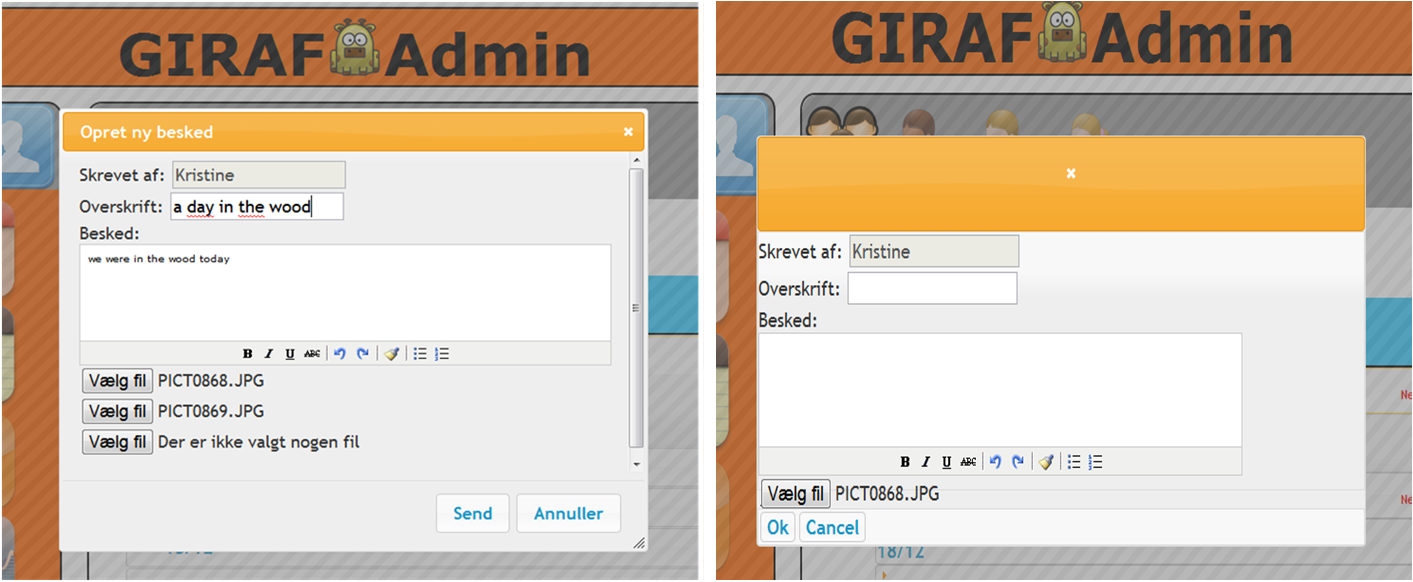
\includegraphics[width=1.00\textwidth]{img/createmessage.png}
	\caption{Create message from the contact book in two versions}
	\label{fig:createmessage}
\end{figure}

In the beginning of the interview she showed us a standard information sheet that contained the child's name, the parents' name and contact information. The current contact book has this sheet in the first page and Kristine though that it also should be included in the digital contact book. However, the sheet will not be placed with the contact book, and she suggested that a button among the other applications' administrators like the Settings button from the first prototype. But we would rather place the information with the other information about the child. 

During the interview she expressed that they rarely did edit pictures before printing, but if they were to upload a picture in a message and easily had access to quick rotation, crop, enlarge/reduce size of the picture then she would probably use it, however, then she would also need an undo button. These functions would be nice to have, but it would not be a priority to be implemented.
From our prototype it was not clear that it would be a closed system, where the kindergarten teachers and parents would have to login before they would be able see or write in the contact book. She thought this very important because the information in the contact book is very sensitive information and the personal Data Protection Act%(persondataloven?)
 covers this area. 

Kristine pointed that now when a child moves on from the kindergarten the child always gets copy of his/hers contact book. If this digital contact book were used instead this tradition would be lost, therefore she suggested that the user e.g. were able to print the contact book so it was not lost afterwards since Birken are not allowed to have these information indefinitely because of the personal Data Protection Act. The solution to this problem should then be studied further.

After the interview we also wanted to have a start page with general information about the meetings and news from Birken to the parents. Kristine first talked about this information in relation to the calendar which only is represented by an icon in the prototype, but that calendar was only supposed as the child's calendar so the other solution was preferred.

\section{The last paper prototype}
In the last primitive paper prototype of the design the menu has changed to two vertical menu, where the user needs to click on an application, a child and then press a go-button to get the application for a child or all children. This is shown in the Figure \vref{fig:calendar} in which the application aSchedule's administrator for Jack is called, however we never implemented an administrator module for aSchedule. When this design was evaluated we thought it would be easier to understand and implement if the user should choose a child or a group of children first and then choose an application, because the applications' administrator depends on the installed applications on the child's device. The go-button was not necessary and was abandoned, while the button Settings was also abandoned as mentioned earlier.

\begin{figure}[!ht]
	\centering
		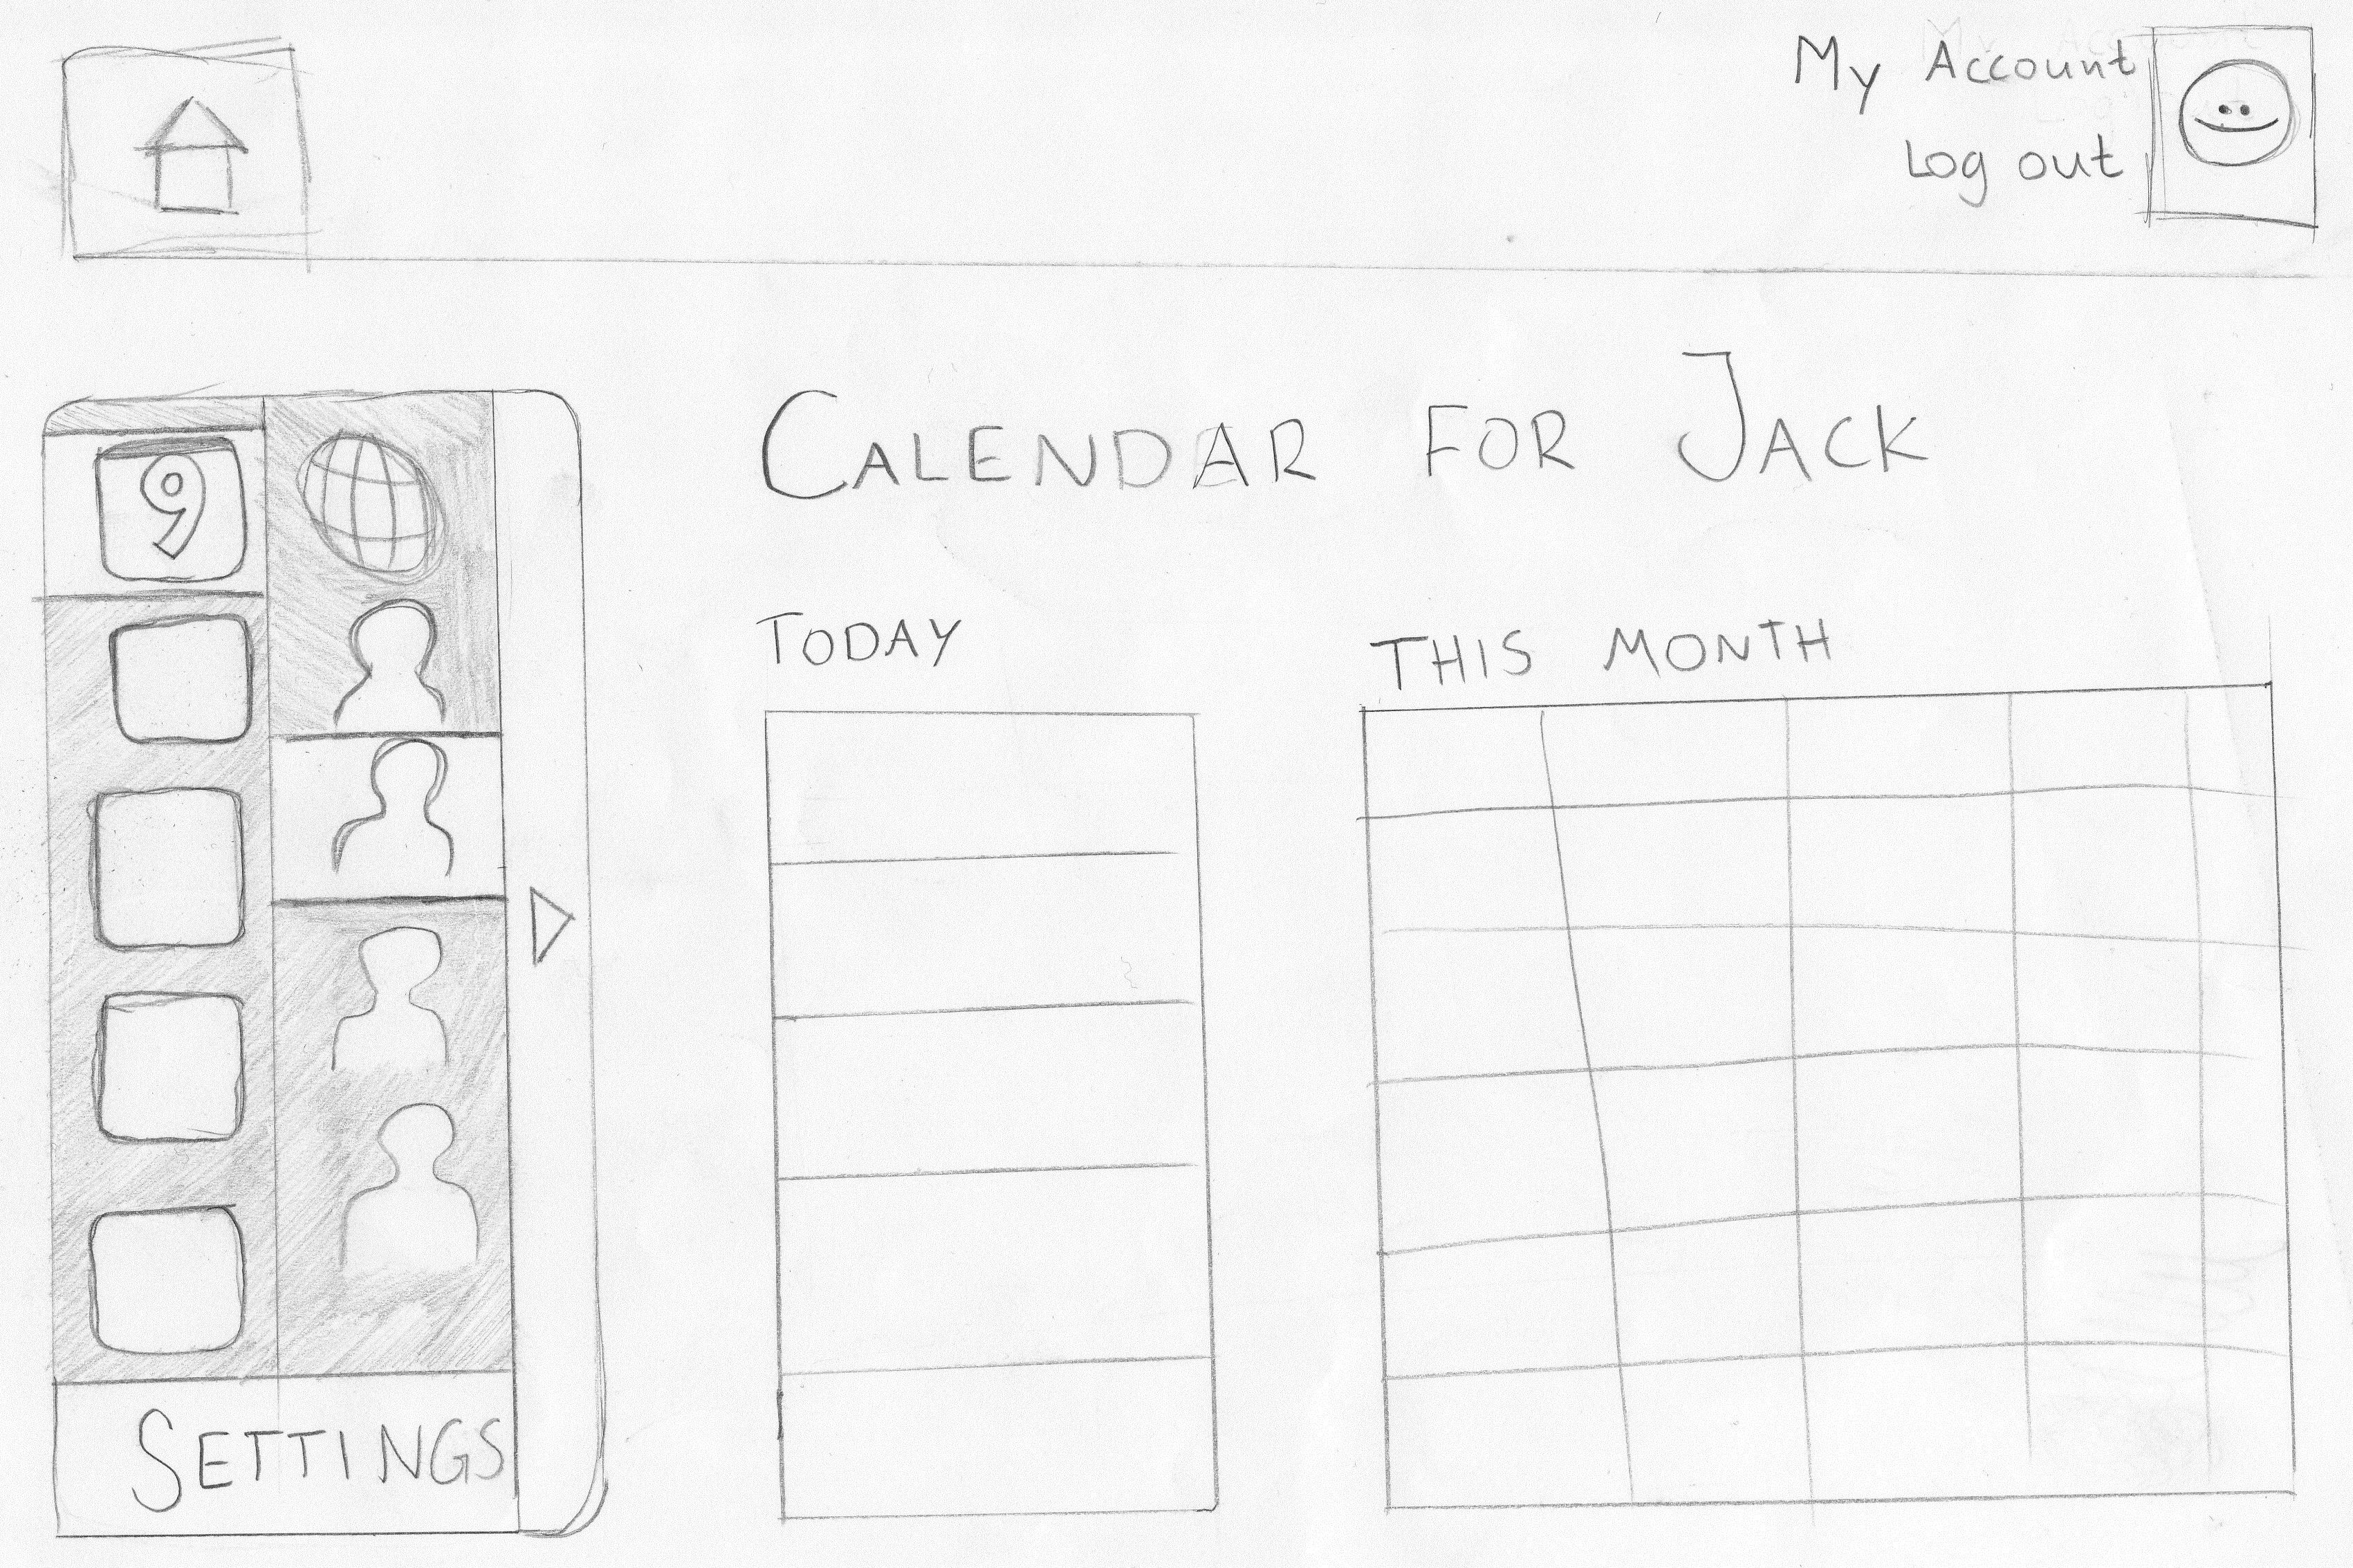
\includegraphics[width=0.60\textwidth]{img/calendar.jpg}
	\caption{Paper prototype of aSchedule's administration application and general design}
	\label{fig:calendar}
\end{figure}

  
In the top-left corner of the prototype is the homepage button which page should contain general information and news from the kindergarten, this was one of the changes made as a result of the interview with Kristine. In the top-right corner should be a logout button and My Account button, which leads to the personal information that is show in Figure \vref{fig:myAccount}. 
\begin{figure}[!ht]
	\centering
		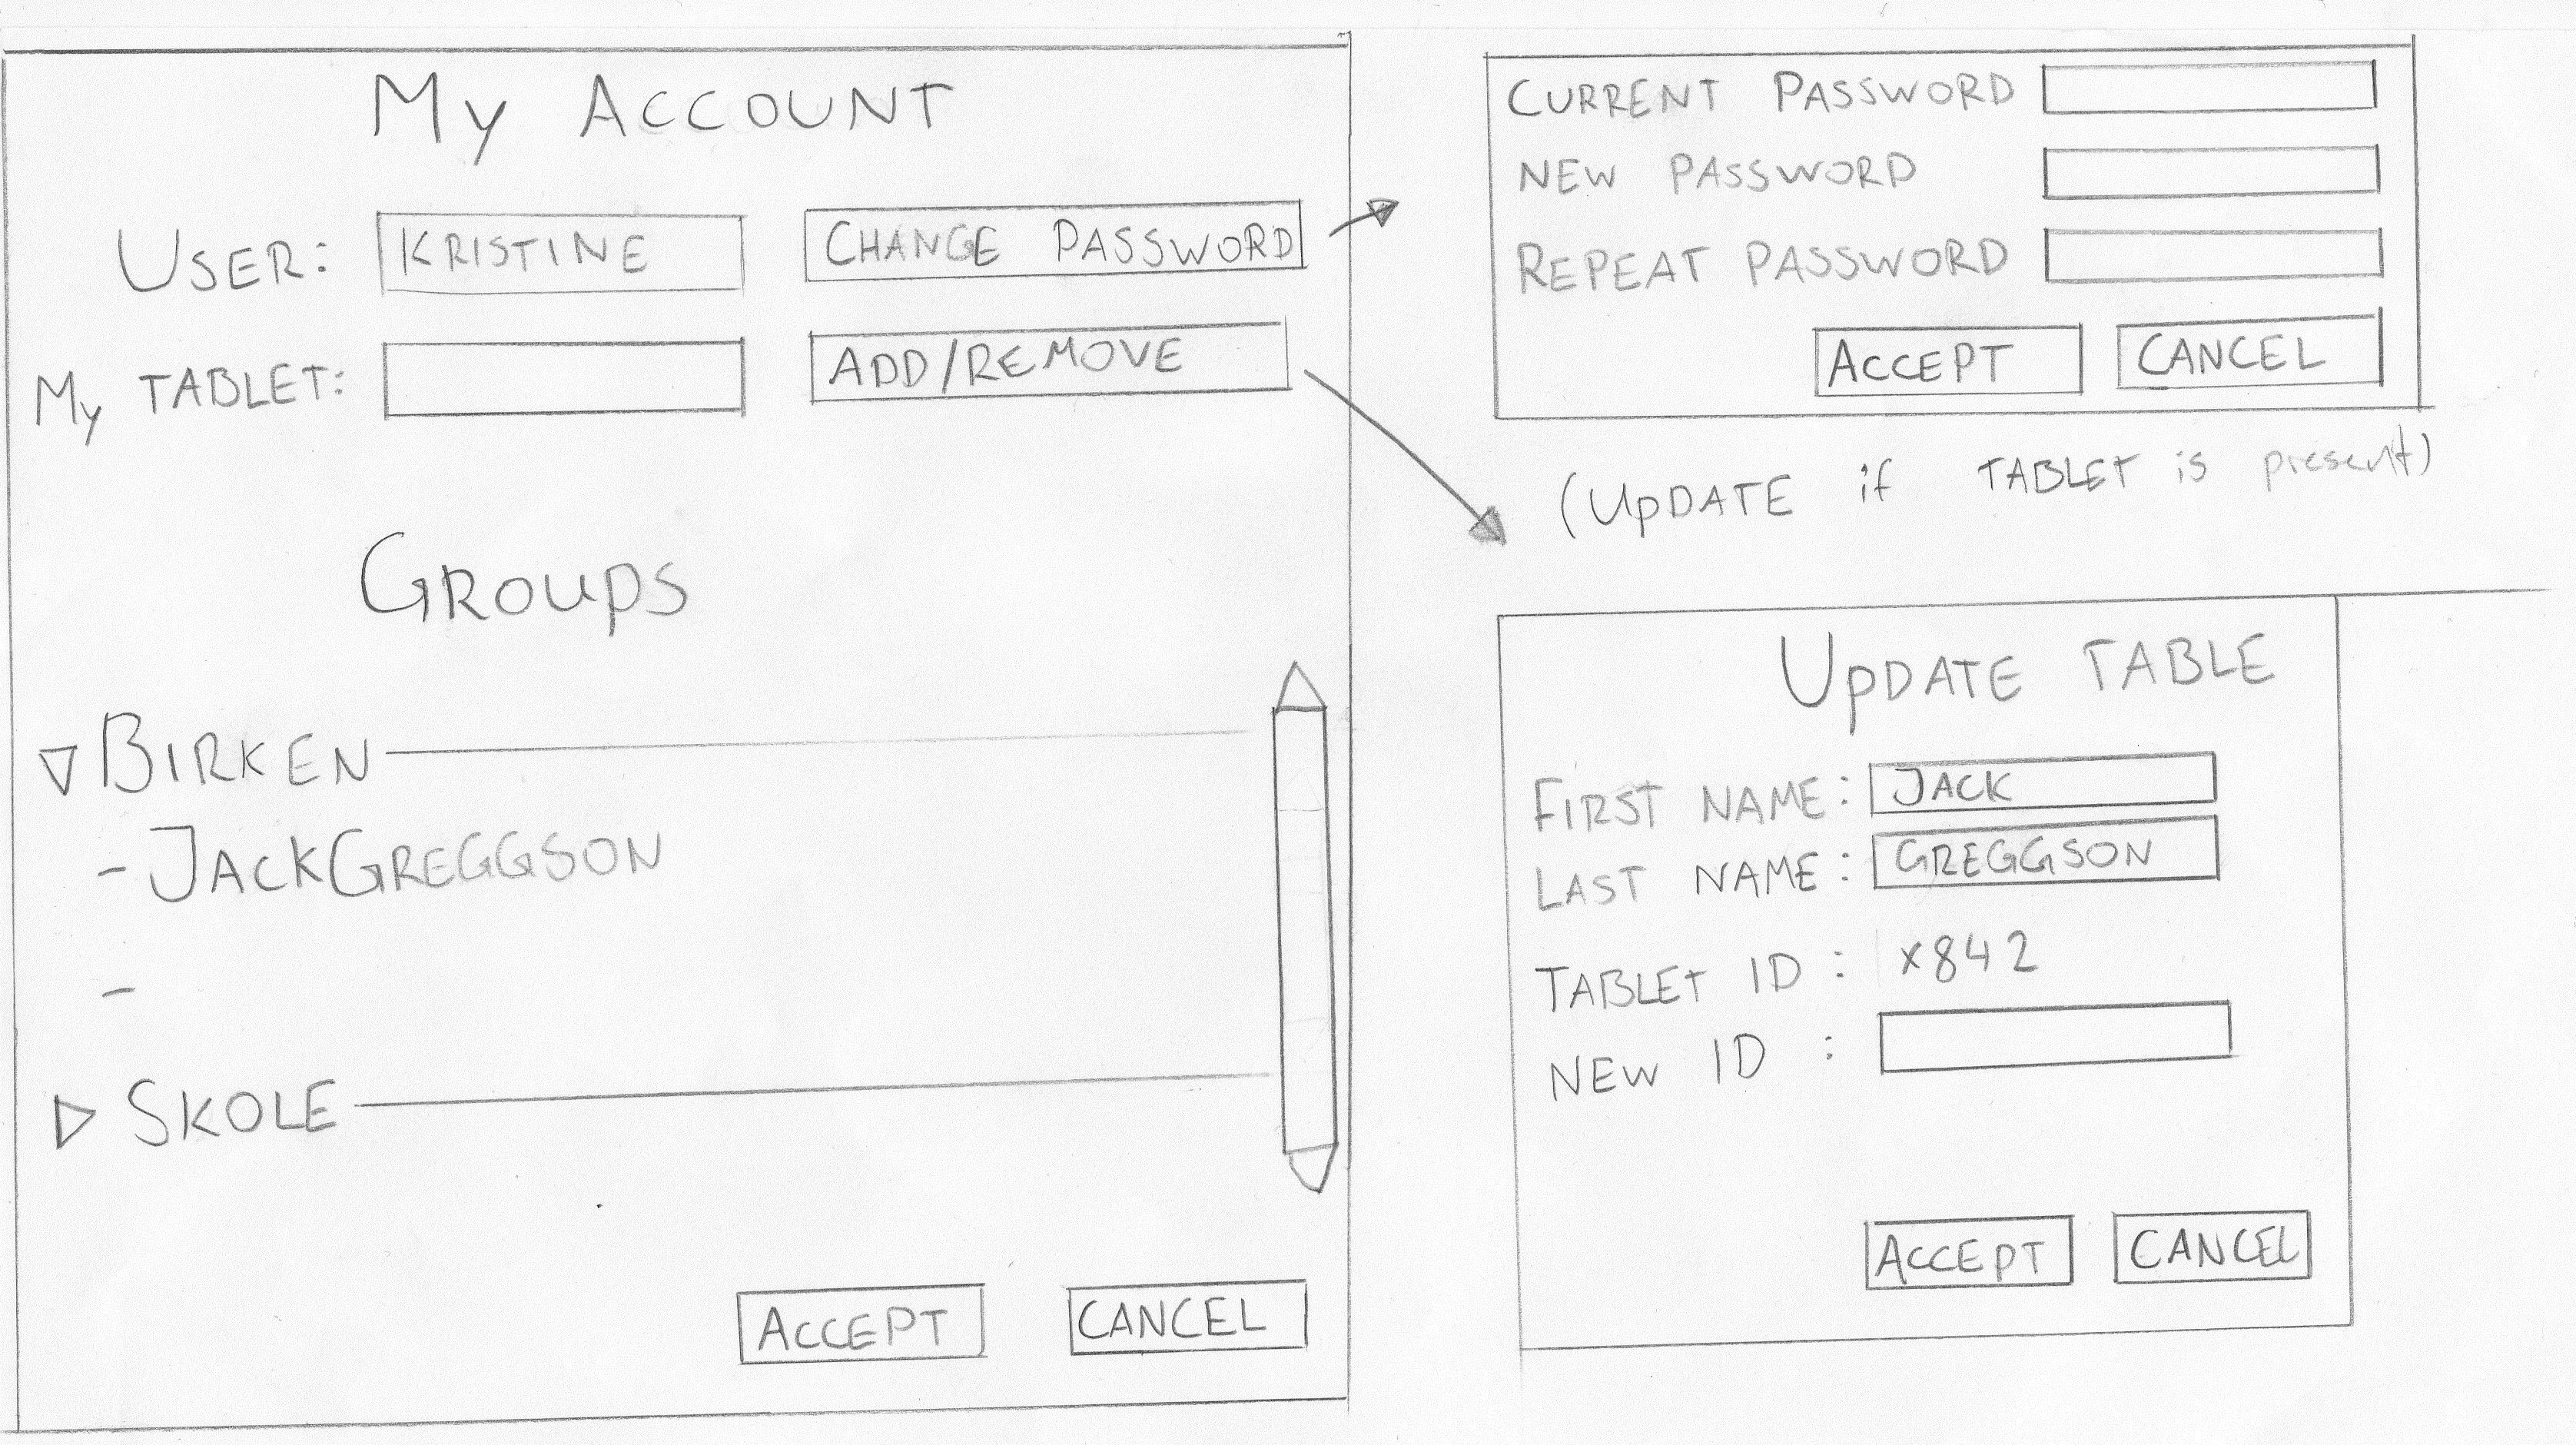
\includegraphics[width=0.60\textwidth]{img/myAccount.jpg}
	\caption{Design of My Account}
	\label{fig:myAccount}
\end{figure}


In this prototype design there are only one page and two pop up boxes, in the first can the user change his/hers password and in the other the user can add/update or delete a device. On the My Account page the user could also see or update devices in a group, however, this design is confusing. This design was not thought through because the field My Tablet could be the users own mobile device, and in the beginning it was meant as his/hers child's mobile device and in both cases the user could have more than one mobile devices that should be registered but cannot in this design. 

The group under My Account is needed, because the user of this administration program could both have access to use this tool privately and work-related, such that the user is parent to an autistic child and is also kindergarten teacher for some other autistic children. This mean groups would be necessary when the user wants to change something on all but his/hers child's device without repeating the same process on all the other children's devices. The design missing something that indicates, how the user can add a device to a group. In the evaluation of this prototype it was also decided that My Account also should contain the child's personal information and device. In the implementation it was also decided that user information, group and child plus child's device should be under different tabs.   
 
\section{The final design}
In Figure \vref{fig:finalDesign} is the design we have used in the  implementation. It is very similar to the last paper prototype and the HTML prototype. Depending on the number of devices the user can administer, will the green menu have a button with picture and name of the child to which device belongs. In the pink menu would all the applications on the child's device be listed with the application's name and icon which is missing in the figure. The contact book's design has a minor change which is when the user is to create a new message which is no longer a light box, but it unfolds when pressing the "Nyt Indl�g" folder.  

\begin{figure}[!ht]
	\centering
		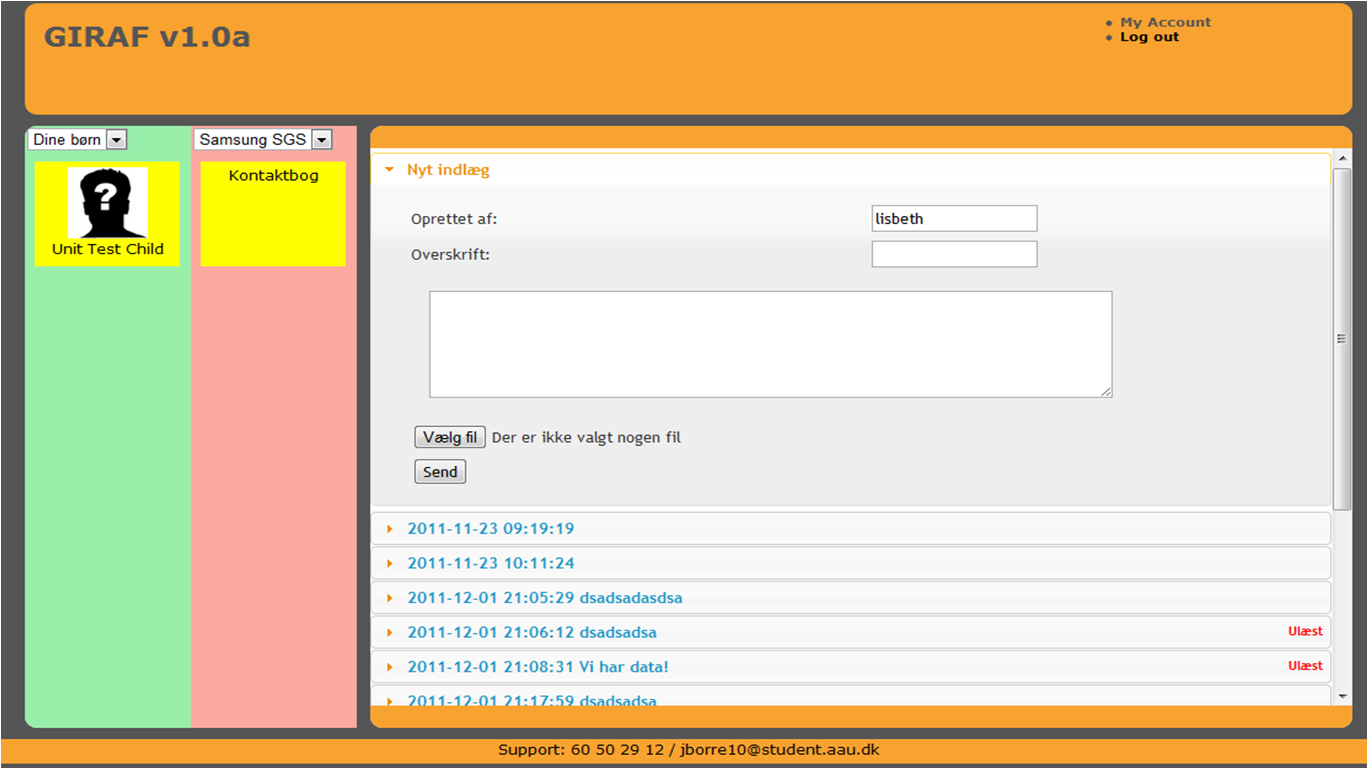
\includegraphics[width=0.90\textwidth]{img/finalDesign.png}
	\caption{Screenshort of the implemented design}
	\label{fig:finalDesign}
\end{figure}

